\documentclass[14pt, titlepage, a4paper]{extarticle} %comment
\usepackage{fancyvrb}
\usepackage[utf8]{inputenc}
\usepackage[T2A]{fontenc}
\usepackage[russian]{babel}
\usepackage{amssymb, amsfonts}
\usepackage{amsmath}

\usepackage{graphicx}

\usepackage{lipsum}
\usepackage{style}
\textwidth 16cm
\textheight 25cm
\oddsidemargin -2.5mm
\evensidemargin -3mm
\topmargin -20mm
\parindent 1.25cm

\usepackage{comment}
%\usepackage{autonum}
\usepackage{amsthm}
\newtheorem{theorem}{Теорема}
\newtheorem{definition}{Опредление}
\newtheorem{corollary}{Следствие}
\newtheorem{lemma}{Лемма}

\begin{document}
	
	%%%%%%%%%%%%%%%%%%%%PAGE%1%%%%%%%%%%%%%%%%%%%%
	%%%%%%%%%%%%%%%%%%%Вкладка%%%%%%%%%%%%%%%%%%%%
	
	\begin{center}
		ЗАДАНИЕ НА КУРСОВОЙ ПРОЕКТ\\
		по дисциплине «Численные методы»
	\end{center}
	
	~\\	
	Ф.И.О. \uline{\vspace{10pt} Бобров И.И., Игнатьев М.В., Абдуллаев Т.М.~~~~~~~~~~~}\\
	~\\
	~\\
	ТЕМА курсового проекта
	
	~\\
	Рекуррентные формулы и интегрирование по Ромбергу.
	\\
	~\\
	~\\
	ФОРМУЛИРОВКА  задания:
	
	\begin{itemize}
		\item Создать алгоритм решения поставленной задачи, реализовать его, протестировать программы;
		\item Оформить и представить итоги проделанной работы в виде отчета;
		\item Сформулировать выводы по полученным решениям, отметить достоинства и недостатки методов.
	\end{itemize}

	~\\
	РУКОВОДИТЕЛЬ проекта\uline{\hspace{80pt}}/ Пак Т.В./\\	
	\\
	~\\
	ДАТА ВЫДАЧИ задания\uline{~6~ноября~2021~}\\
	\\
	~\\
	СРОК ВЫПОЛНЕНИЯ задания 09.11.2020 – 10.01.2021\\
	\\
	~\\
	Задание получил \uline{Бобров И.И., Игнатьев М.В., Абдуллаев Т.М.}\\
	
	\thispagestyle{empty}
	\newpage
	
	%%%%%%%%%%%%%%%%%%%%PAGE%2%%%%%%%%%%%%%%%%%%%%
	%%%%%%%%%%%%%%%%%%Титульник%%%%%%%%%%%%%%%%%%%
	
	\begin{comment}
	\fefutitlepage{Б8118-01.03.02миопд}{Бобров И.И.}{Игнатьев М.В.}{Абдуллаев Т.М.}{5}
	\defaultfont
	\end{comment}

	%%%%%%%%%%%%%%%%%%%%PAGE%3%%%%%%%%%%%%%%%%%%%%
	%%%%%%%%%%%%%%%%%%Содержание%%%%%%%%%%%%%%%%%%

	\tableofcontents
	\pagebreak
	
	%%%%%%%%%%%%%%%%%%%%PAGE%4%%%%%%%%%%%%%%%%%%%%
	%%%%%%%%%%%%%%%%%%%Введение%%%%%%%%%%%%%%%%%%%
	
	\section*{Рекуррентные формулы и интегрирование по Ромбергу}
	\addcontentsline{toc}{section}{Рекуррентные формулы и интегрирование по Ромбергу.}
	
	\subsection*{Введение}
	\addcontentsline{toc}{subsection}{Введение}
	
	Объектом исследования являются численные методы решения задач численного интегрирования.\\
	\textit{Цель работы} – ознакомиться с численными рекуррентными формулами и методами интегрирования, решить предложенные типовые задачи, сформулировать выводы по полученным решениям, отметить достоинства и недостатки методов, приобрести практические навыки и компетенции, а также опыт самостоятельной профессиональной деятельности, а именно:
	\begin{itemize}
		\item создать алгоритм решения поставленной задачи и реализовать его, протестировать программы;
		\item освоить теорию вычислительного эксперимента; современных компьютерных технологий; 
		\item приобрести навыки представления итогов проделанной работы в виде отчета, оформленного в соответствии с имеющимися требованиями, с привлечением современных средств редактирования и печати.	
	\end{itemize}
	Работа над курсовым проектом предполагает выполнение следующих задач:
	\begin{itemize}
		\item дальнейшее углубление теоретических знаний обучающихся и их систематизацию;
		\item получение и развитие прикладных умений и практических навыков по направлению подготовки;
		\item овладение методикой решения конкретных задач;
		\item развитие навыков самостоятельной работы;
		\item развитие навыков обработки полученных результатов, анализа и осмысления их с учетом имеющихся литературных данных;
		\item приобретение навыков оформления описаний программного продукта;
		\item повышение общей и профессиональной эрудиции.
	\end{itemize}

	
	\pagebreak
	
	%%%%%%%%%%%%%%%%%%%%PAGE%5%%%%%%%%%%%%%%%%%%%%
	%%%%%%%%%%%%%%%%Основная%часть%%%%%%%%%%%%%%%%
	%%%%%%%%%%%%%%%Постановка%задачи%%%%%%%%%%%%%%%
	
	\subsection*{Основная часть}
	\addcontentsline{toc}{subsection}{Основная часть}
	
	%\subsubsection*{Постановка задач}
	%\addcontentsline{toc}{subsubsection}{Постановка задач}
	
	Приближения имеют высокую точность, если использовать большее количество подынтервалов. Сколько их следует выбрать? Ответить на этот вопрос может помочь процесс последовательного
	выбора двух, четырех и т. д. подынтервалов, пока не будет достигнута требуемая точность. Сначала необходимо сгенерировать последовательность {T(J)} формул трапеций для приближений. Как только число подынтервалов удваивается, число значений функции также приблизительно удваивается, поскольку функцию нужно вычислять во всех предыдущих точках и во всех средних точках предыдущих подынтервалов (рис 1). В теореме 7.4 объясняется, как удалить лишние вычисления функции и сложения.
	
	\begin{figure}[h]
		\centering
		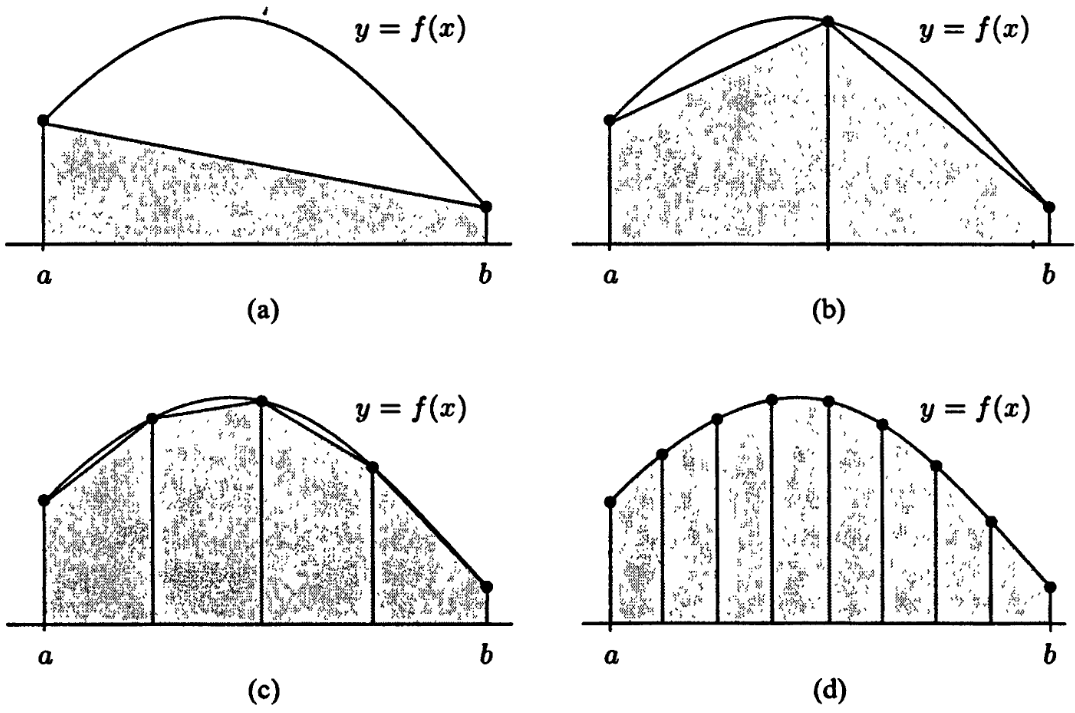
\includegraphics[width=400pt]{pic1.png}
		\caption{\textbf{(a)} $T(0)$ — площадь под $2^0 = 1$ трапецией, \textbf{(b)} $T(1)$ — площадь под		$2^1 = 2$ трапециями, \textbf{(с)} $Т(2)$ — площадь под $2^2 = 4$ трапециями, \textbf{(d)} $Г(3)$ — площадь под $2^3 = 8$ трапециями}
	\end{figure}
	
	\begin{theorem}\label{th:7.4}
		\textbf{(последовательные формулы трапеций).} Предположим, что $J \geqslant 1$ и точки \{$x_k = a + kh$\} делят интервал $\left[a; b\right]$ на $2^J = 2M$ подынтервалов с одинаковым шагом $h = (b-a)/2^J$. Формулы трапеций $T(f,h)$ и $T(f,2h)$ удовлетворяют соотношению
		\begin{equation}\label{eq:1}
			T(f,h)=\frac{T(f,2h)}{2} + h\sum_{k=1}^{M}f(x_{2k-1})
		\end{equation}
	\end{theorem}
	
	\begin{definition}\label{df:7.3}
		\textbf{(последовательность формул трапеций).} Определим $T(0) = (h/2)(f(a)+f(b))$ как формулу трапеций с шагом длины $h = b - a$. Затем для каждого $J\ge1$ определим $T(J)=T(f,h)$, где $T(f,h)$ - формула трапеций с шагом длинны $h = (b-a)/2$.
	\end{definition}
	
	\begin{corollary}\label{cr:7.4}
	\textbf{(рекуррентная формула трапеций).} Начнем с $Т(0) = (h/2) х (f(a) + f(b))$. Тогда последовательность формул трапеций ${T(J)}$ генерируется согласно рекуррентной формуле
		\begin{equation}\label{eq:2}
			T(J) = \frac{T(J-1)}{2}+ h\sum_{k-1}^{M}f(x_{2k-1})~~\text{для} J = 1, 2,~...~.
		\end{equation}
	где $h=(b-a)/2^J$ и ${x_k = a + kh}$.
	\end{corollary}
	
	
	\begin{theorem}\label{th:7.5}
		\textbf{(рекуррентная формула Симпсона).} Предположим, что $\{T(J)\}$ - последовательность формул трапеций, сгенерированная согласно следствию (\ref{cr:7.4}). Если $J\ge1$ и $S(J)$ - формула Симпсона для $2^J$ подынтервалов $[a;b]$, то $S(J)$ и формулы трапеций $T(J-1)$ и $T(J)$ удовлетворяют соотношению
		\begin{equation}\label{eq:7}
			S(J) = \frac{4T(J)-T(J-1)}{3}~~~\text{для}~J = 1,2,~...~.
		\end{equation}
	\end{theorem}
	
	
	\begin{theorem}\label{th:7.6}
		\textbf{(рекуррентная формула Буля).} Предположим, что $\{S(J)\}$ - последовательность формул Симпсона, сгенерированная согласно теореме (\ref{th:7.5}). Если $J\ge2$ и $B(J)$ - формула Буля для $2^J$ подынтервалов интервала $[a;b]$, то $B(J)$ и формулы Симпсона $S(J-1)$ и $S(J)$ удовлетворяют соотношению
		\begin{equation}\label{eq:14}
			B(J) = \frac{16S(J)-S(J-1)}{15}~~~\text{для}~J=2,3,~...~.
		\end{equation}
	\end{theorem}
	
	%%%%%%%%%%%%%%%%%%%%%%%%%%%%%%%%%%%%%%%%%%%%%%%%%%%%%%%%%%%%%%%%%%%%%%%%%%%%%%%%%%%%%%%
	\textbf{Интегрирование по Ромбергу}
	
	
	\begin{lemma}
		\textbf{(улучшение Ричардсона для интегрирования по Ромбергу).} Заданы два приближения, $R(2h,К—1)$ и $R(h,K—1)$, для величины $Q$, которые
		удовлетворяют равенствам
		\begin{equation}\label{eq:28}
			Q = R(h,K-1)+c_1h^{2K}+c_2h^{2K+2}+...
		\end{equation}
		и
		\begin{equation}\label{eq:29}
			Q = R(2h,K-1)+c_14^Kh^{2K}+c_24^{K+1}h^{2K+2}+...~.
		\end{equation}
		Улучшенное приближение имеет вид
		\begin{equation}\label{eq:30}
			Q = \frac{4^KR(h,K-1)-R(2h,K-1)}{4^K-1}+O(h^{2K+2}).
		\end{equation}
	\end{lemma}


	\begin{definition}\label{df:7.4}
		Определим последовательность ${R(J,K):J\ge K}^{\infty}_{J=0}$ формул квадратуры для $f(x)$ на интервале $[a;b]$ следующим образом.
		\begin{eqnarray}
			\nonumber
			R(J,0) &=& T(J)~~~\text{для}~J\ge 0\text{, последовательная формула трапеций.}\\
			\nonumber
			R(J,1) &=& S(J)~~~\text{для}~J\ge 1\text{, последовательная формула Симпсона.}\\
			\label{eq:31}
			R(J,2) &=& B(J)~~~\text{для}~J\ge 2\text{, последовательная формула Буля.}
		\end{eqnarray}
	\end{definition}

	%%%%%%%%%%%%%%%%%%%%%%%%%%%%%%%%%%%%%%%%%%%%%%%%%%%%%%%%%%%%%%%%%%%%%%%%%%%%%%%%%%%%%%%
	%%%%%%%%%%%%%%%%%%%%%%%%%%%%%%%%%%%%Мусор%%%%%%%%%%%%%%%%%%%%%%%%%%%%%%%%%%%%%%%%%%%%%%
	%%%%%%%%%%%%%%%%%%%%%%%%%%%%%%%%%%%%%%%%%%%%%%%%%%%%%%%%%%%%%%%%%%%%%%%%%%%%%%%%%%%%%%%

	Вот это обычный текст за пределами теорем и определений. Вот это обычный текст за пределами теорем и определений. Вот это обычный текст за пределами теорем и определений. Вот это обычный текст за пределами теорем и определений. Вот это обычный текст за пределами теорем и определений. Вот это обычный текст за пределами теорем и определений. Вот это обычный текст за пределами теорем и определений. Вот это обычный текст за пределами теорем и определений. Вот это обычный текст за пределами теорем и определений. 
	
	\begin{theorem}\label{th:7}
		\textbf{(точность интегрирования по Ромбергу).} Предположим, что $f \in C^{2K+2}[a;b]$. Тогда ошибка усечения для приближения Ромберга задается формулой
		\begin{equation}\label{eq:34}
			\int_{a}^{b}{f(x)dx} = R(J,K) + b_Kh^{2K+2}f^{(2K+2)}(c_{J,K}) = R(J,K) + O(h^{2K+2}),
		\end{equation}	
		где $h = (b-a)/2^J,~b_K$ - постоянная, зависящая от $K$, и $c_{J,K}\in[a;b].$
	\end{theorem}
	
	
	
	%\subsubsection*{Описание алгоритмов решения}
	%\addcontentsline{toc}{subsubsection}{Описание алгоритмов решения}
	
	\subsubsection*{Вычислительный эксперимент}
	\addcontentsline{toc}{subsubsection}{Вычислительный эксперимент}
	
	
	
	\pagebreak
	
	%%%%%%%%%%%%%%%%%%%%%%%%%%%%%%%%%%%%%%%%%%%%%%
	%%%%%%%%%%%%%%%%%%%%PAGE%?%%%%%%%%%%%%%%%%%%%%
	%%%%%%%%%%%%%%%%%%Заключение%%%%%%%%%%%%%%%%%%
	
	\subsection*{Заключение}
	\addcontentsline{toc}{subsection}{Заключение}
	
	В результате работы над курсовым проектом приобрел практические навыки владения:
	\begin{itemize}
		\item современными численными методами решения задач математической экономики;
		\item основами алгоритмизации для численного решения задач математической экономики на одном из языков программирования;
		\item инструментальными средствами, поддерживающими разработку программного обеспечения для численного решения задач математической экономики; 
	\end{itemize}
	а также навыками представления итогов проделанной работы в виде отчета, оформленного в соответствии с имеющимися требованиями, с привлечением современных средств редактирования и печати.
	
	\pagebreak

	%%%%%%%%%%%%%%%%%%%%PAGE%?%%%%%%%%%%%%%%%%%%%%
	%%%%%%%%%%%%%%%%%%%Источники%%%%%%%%%%%%%%%%%%
	
	\subsection*{Список используемых источников}
	\addcontentsline{toc}{subsection}{Источники}
	
	\textbf{Источники}
	\begin{enumerate}
		\item Численные методы. Использование Matlab. Третье издание. Джон Г. Мэтьюз Издательский дом $"$Вильямс$"$ 2001
	\end{enumerate}
	
	\pagebreak
	
	%%%%%%%%%%%%%%%%%%%%PAGE%?%%%%%%%%%%%%%%%%%%%%
	%%%%%%%%%%%%%%%%%%Приложения%%%%%%%%%%%%%%%%%%
	
	\subsection*{Приложения}
	\addcontentsline{toc}{subsection}{Приложения}
	
	\pagebreak	
	
	
\end{document}